\chapter{What is computer hardware?}

\section{Inside a personal computer}

All though the term \emph{personal computer} (PC) is commonly known, a formal definition is good to clear up any confusion. Knowledge of basic computer components (CPU, GPU, etc.) are going to be assumed.

\begin{definition}[Personal computer]
    A \textbf{personal computer} is a multipurpose whose size, capabilities, and price make it appropriate for individual use. They are intended to be used by an end user, rather than a computer expert or technician.
\end{definition}

Looking at the internal components of a PC, we generally see a \textbf{motherboard} upon which are an array of different components, a cooling system (fans), and an interface between the PC and external components (such as USB).

\begin{definition}[Motherboard]
    A \textbf{motherboard} is the main printed circuit board found in PCs, they allow communication between many of the crucial electronic components that make up a computer.

\end{definition}

\begin{remark}
    Traditionally, the motherboard is separated into two parts: the \textbf{northbridge} and the \textbf{southbridge}. The \textbf{northbridge} is the chipset that handles fast communications to and from the central processing unit (CPU) to components such as the primary memory and the graphical processing unit (GPU). The \textbf{southbridge} handles slower communications to components such as peripherals (mouse, keyboard, etc.) and networks. Nowadays, the northbridge is increasingly becoming part of the CPU itself.
\end{remark}

\begin{definition}[Bus]
    \textbf{Buses} are wires from which communications between components are sent.
\end{definition}
 
\section{Silicon chips}

\begin{definition}[Integrated circuit]
    An \textbf{integrated circuit} is a set of electronic circuits on one small flat piece of semiconductor material (typically silicon).
\end{definition}
 
\begin{definition}
    The \textbf{central processing unit} (CPU) is where the instructions of computer programs are carried out. It is an \textbf{integrated circuit} (IC) which consists of millions of \textbf{transistors} (defined later) interconnected by microscopic wires on a footprint of around \SI{1}{\centi\meter\squared}.
\end{definition}

\begin{remark}
    We use silicon to make CPUs because the chemical and electrical semiconductor properties of silicon make it ideal for building transistors.
\end{remark}

The CPU is etched onto a wafer of silicon. The following are the typical steps in the production of a CPU:

\begin{enumerate}
    \item a silicon ingot is fed through a slicer to make several blank wafers;
    \item through various processing steps the blank wafers are made into \textbf{patterned wafers};
    \item the patterned wafers are then tested and only functional wafers are processed in a dicer, this is the machine that etches onto silicon wafer to make a \textbf{die}; and
    \item the dies are then tested and each error-free die is cut and mounted into a package with the die's pads connected to the package pins such that direct contact with other components within the CPU is possible.
\end{enumerate}

A high proportion of the silicon wafers and dies are defective which is one of the factors that cause CPUs to be so expensive.

\begin{proposition}[Moore's law]
    \textbf{Moore's law} is the observation that the number of transistors in a dense integrated circuit doubles about every two years.
\end{proposition}

\begin{definition}
    A \textbf{multicore processor} is an IC with multiple CPUs etched on. These cores share some components such as main memory.
\end{definition}

Recently, it has been speculated whether Moore's law will hold for the future due to us reaching the physical limit for how small we can make transistors. Additionally, as the transistor density in an integrated circuit increases, the power dissipation also increases. This has driven growth of multicore processors where one CPU with a high clock speed is replaced by many CPUs with lower clock speed.

\section{Gates}

\begin{definition}
    A \textbf{transistor}, or more specifically a \textbf{bipolar junction transistor} (BJT) is a semiconductor device used to amplify and switch electronic signals. Every BJT has
    \begin{enumerate}
        \item a \textbf{collector}, from which electricity can flow;
        \item an \textbf{emitter}, to which electricity can flow; and
        \item a \textbf{base}, to which a voltage can be applied.
    \end{enumerate}
    
    There are two types of BJT transistors:
    \begin{enumerate}
        \item \textbf{NPN transistor}, if the base voltage is high then current can flow from the collector to the emitter, otherwise, there is no current flow; and
        \item \textbf{PNP transistor}, if the base voltage is low then current can flow, otherwise, there is no current flow.
    \end{enumerate}
\end{definition}

% some diagrams of transistors (NPN vs PNP) and then go onto the gates etc.

Transistors can be compiled together to make \textbf{logic gates}, as defined below.

\begin{definition}
    A \textbf{logic gate} is a physical device that implements a Boolean function, that is, a small circuit that takes boolean inputs, $1$ and $0$, which are interpreted as being a high or low voltage respectively, and produces a boolean output (or outputs).
\end{definition}

There are three fundamental gates: NOT-gates, AND-gates, and OR-gates, as defined below.

\begin{definition}[NOT-gate]
    A NOT-gate (or inverter) implements logical negation, the truth table is shown below.
    \begin{center}
        \begin{tabular}{ccc}
                \toprule
                $A$ & NOT $A$ \\
                \midrule
                0 & 1 \\ 
                1 & 0 \\
                \bottomrule
        \end{tabular}
    \end{center}
\end{definition}

\begin{definition}[AND-gate]
    An AND-gate implements logical conjunction, the truth table is shown below.
    \begin{center}
        \begin{tabular}{ccc}
                \toprule
                $A$ & $B$ & $A$ AND $B$ \\
                \midrule
                0 & 0 & 0 \\ 
                0 & 1 & 0 \\ 
                1 & 0 & 0 \\ 
                1 & 1 & 1 \\
                \bottomrule
        \end{tabular}
    \end{center}
\end{definition}

\begin{definition}[OR-gate]
    An OR-gate implements logical disjunction, the truth table is shown below.
    \begin{center}
        \begin{tabular}{ccc}
                \toprule
                $A$ & $B$ & $A$ OR $B$ \\
                \midrule
                0 & 0 & 0 \\ 
                0 & 1 & 1 \\ 
                1 & 0 & 1 \\ 
                1 & 1 & 1 \\
                \bottomrule
        \end{tabular}
    \end{center}
\end{definition}

\begin{figure}
    \centering
        % NOT gate
        \begin{circuitikz}
            \draw
    			(0,0) node[not port] (not) {}
    			(not.in) node[left] {$A$}
    			(not.out) node[right] {NOT $A$}
    		;
        \end{circuitikz}
        \hspace{2em}
        % AND gate
        \begin{circuitikz}
            \draw
    			(0,0) node[and port] (and) {}
    			(and.in 1) node[left] {$A$}
    			(and.in 2) node[left] {$B$}
    			(and.out) node[right] {$A$ AND $B$}
    		;
        \end{circuitikz}
        \hspace{2em}
        % OR gate
        \begin{circuitikz}
            \draw
    			(0,0) node[or port] (or) {}
    			(or.in 1) node[left] {$A$}
    			(or.in 2) node[left] {$B$}
    			(or.out) node[right] {$A$ OR $B$}
    		;
        \end{circuitikz}
    \caption{The symbols used for NOT, AND, and OR gates}
    \label{fig:logic_gate_symbols}
\end{figure}

Even though logically we view these three gates as fundamental, when building circuits we find that NAND-gates (NOT AND) can be thought of as the fundamental logical as every logic gate can built out of a NAND-gates and we can effectively make very small NAND-gates.

\begin{theorem}
    Let $f : \mathbb Z_2^n \to \mathbb Z_2$. Then we can construct a circuit that computes $f$.
\end{theorem}

\begin{example}[Adders]
    Let's apply our theorem above, let's consider addition of two binary numbers. First we will consider one digit addition. Let $x, y \in \mathbb Z_2$, we want to compute $x + y$. As this can be 2 digits, we must have outputs $s$ and $c$ (carry). We can just follow logical reasoning to deduce
    \[
        c =
        \begin{cases}
            1 & \text{if} \; x = 1, \, y = 1 \\
            0 & \text{else}
        \end{cases}
    \]
    and
    \[
        s =
        \begin{cases}
            1 & \text{if} \; x = 1, \, y = 0 \; \text{or} \; x = 0, \, y = 1 \\
            0 & \text{else}
        \end{cases}
        ;
    \]
    hence, we can build a circuit as follows.
    \begin{center}
        \begin{circuitikz}
            \coordinate (O) at (0,0);
            \draw
                (2,2) node[and port] (and1) {}
                (2,0) node[or port] (or1) {}
                (3.5,1) node[not port] (not1) {}
                (or1.out) ++ (4,0.28) node[and port] (and2) {}
                (and1.in 1) node[left, xshift=-1em] (x) {$x$}
                (and1.in 2) node[left, xshift=-1em] (y) {$y$}
                (x) -| (or1.in 1)
                (y) ++ (0.8, 0) -- (y)
                (or1.in 2) ++ (-0.2, 0) -- (or1.in 2) 
                (or1.in 2) ++ (-0.2, 0) |- (y)
                (and1.out) -| (not1.in)
                (and1.out) ++ (4.1, 0) node[right] (s) {$s$} -- (and1.out) 
                (not1.out) -- (and2.in 1)
                (or1.out) -- (and2.in 2)
                (and2.out -| s) node (c) {$c$}
            ;
        \end{circuitikz}
    \end{center}
    We can now use this circuit to build a full adder which can compute the sum of three binary digits.
    \begin{center}
        \begin{circuitikz}
            \draw 
                (1, 0) rectangle (3, 1)
                (4, 2) rectangle (6, 3)
            ;
            \node at (2, 0.5) {half-adder};
            \node at (5, 2.5) {half-adder};
            \draw
                (9, 1.5) node[or port] (or1) {}
                (0, 2.7) node[left] {$x$} -- (4, 2.7)
                (0, 0.7) node[left] {$y$} -- (1, 0.7)
                (0, 0.3) node[left] {$z$} -- (1, 0.3)
                (3, 0.7) node[right, xshift = 1.4em] {sum} -- (3.5, 0.7) -- (3.5, 2.3) -- (4, 2.3)
                (3, 0.3) node[below right] {carry} -- (6, 0.3) |- (or1.in 2)
                (6, 2.3) node[below right, xshift = 1.4em] {carry} -- (6.5, 2.3) |- (or1.in 1)
                (6, 2.7) node[above right] {sum} -- (10, 2.7) node[right] {$s$}
                (or1.out) -- (10, 1.5) node[right] {$c$}
            ;
        \end{circuitikz}
    \end{center}
    We can now combine full adders to add $n$-bit numbers.
    
    \begin{center}
        \begin{circuitikz}
            \draw 
                (1, 0) rectangle (3, 1)
                (4, 2) rectangle (6, 3)
                (7, 4) rectangle (9, 5)
            ;
            \node at (2, 0.5) {half-adder};
            \node at (5, 2.5) {full-adder};
            \node at (8, 4.5) {full-adder};
            \draw
                (0, 0.3) node[left] {$x_1$} -- (1, 0.3)
                (0, 0.7) node[left] {$y_1$} -- (1, 0.7)
                (0, 2.5) node[left] {$x_2$} -- (4, 2.5)
                (0, 2.8) node[left] {$y_2$} -- (4, 2.8)
                (0, 4.5) node[left] {$x_3$} -- (7, 4.5)
                (0, 4.8) node[left] {$y_3$} -- (7, 4.8)
                (3, 0.3) -- (10, 0.3) node[right] {$z_1$}
                (3, 0.7) -- (3.5, 0.7) -- (3.5, 2.2) -- (4, 2.2)
                (6, 2.3) -- (10, 2.3) node[right] {$z_2$}
                (6, 2.7) -- (6.5, 2.7) -- (6.5, 4.2) -- (7, 4.2)
                (9, 4.3) -- (10, 4.3) node[right] {$z_3$}
                (9, 4.7) -- (10, 4.7) node[right] {$z_4$}
            ;
        \end{circuitikz}
    \end{center}
\end{example}

\section{Integrated circuit design}

When designing an integrated circuit we have three different levels of design:

\begin{enumerate}
    \item \textbf{functional specification}, this describes what the chip is supposed to do, factors listed will include function, power, speed, and cost;
    \item \textbf{register transfer level}, this describes the exact behaviour of the chip, such as what inputs it will take and the outputs; and
    \item \textbf{physical layout}, this is whow the chip will be printed on silicon, we have a significant amount of testing here to ensure that the chip acts as the register transfer level design states.
\end{enumerate}

To make sure that a chip does as designed, there needs to be a significant amount of testing. 

\begin{definition}[Formal methods]
    \textbf{Formal methods} are a particular kind of mathemetically based technique for the specification, development, and verification of software and hardware systems. 
\end{definition}

The aim of formal methods it to avoid relying on empirical tests and have a robust fondation for our systems. Within formal methods, we have techniques such as \textbf{model checking} and \textbf{computer-aided verification}. 

\begin{definition}[Hardware description language]
    A \textbf{hardware description language} (HDL) is a language whose purpose is the formal description of digital logic circuits. It describes the behaviour of a circuit as well as its design and organisation. HDL can also provide a interface for writing specific tests.
\end{definition}

In contrast to typically programming language, HDLs take into account \textbf{time} and \textbf{concurrency}, two major components in intregrated circuits. 

\section{Memory}

\begin{definition}[Memory]
    \textbf{Memory} refers to the integrated circuits that store information for use in a computer. We can split memory into memory that can be directly accessed by the CPU, \textbf{primary memory}, and data that can not be directly accessed by the CPU, \textbf{secondary memory}.
\end{definition}

\begin{definition}[Hard disk drives]
    \textbf{Hard disk drives} (usually) consists of rapidly rotating disks with magnetic heads which it uses to store data. 
\end{definition}

\begin{definition}[Solid state drives]
    \textbf{Solid-state drives} uses integrated circuits to store data, it has no moving parts and is typically faster than hard disk drives. 
\end{definition}

Hard disk drives and solid state drives are both common secondary storage devices, hard disk drives are typically chosen to store large volumes of data that do not need to be accessed quickly as hard disk drives are cheap (per amount of data stored) and slow. Solid state drives are more typically for holding program files and operating systems as it leads to faster load times. 

\begin{definition}[RAM]
    \textbf{Random access memory} (RAM) is primary storage and takes the form of an integrated circuit and comes in two forms:
    \begin{enumerate}
        \item \textbf{dynamic RAM} (DRAM) is where a bit of data is stored using a transistor and capacitor combination, it is relatively cheap although it needs to be refreshed and can be slow; and
        \item \textbf{static RAM} (SRAM) is where a bit of data is stored by a \textbf{flip-flop} (covered in Computer Systems) which incorporates 4 to 6 transistors, it is fast and stable.
    \end{enumerate}
\end{definition}

\begin{definition}[Caches]
    Cache memory is primary memory that is fast and expensive that is used to store frequently accessed data. We split cache into multiple levels, a level 1 cache (being the highest) usually consists of static RAM and is build directly onto the CPU. Level 2 cache usually also consists of static RAM and might be built onto the CPU, but could also be a short distance away. 
\end{definition}

\section{Microarchitecture}

\begin{definition}[Microarchitecture]
    The \textbf{microarchitecture} of a processor is the organisation of the different components of the process. The three key components that we will look at are:
    \begin{enumerate}
        \item data path;
        \item control; and
        \item cache.
    \end{enumerate}
\end{definition}

\begin{definition}[Datapath]
    This is where most of the processing will be done, it contains the \textbf{arithmetic logic unit} (where calculations are carried out) and a limited number of registers.
\end{definition}

\begin{definition}[Control]
    This controls the processors and communicates with memory and devices, such as to load data into registers or cache.
\end{definition}

\begin{definition}[Cache]
    This is fast memory where frequently used data is stored to be loaded (quickly) into the processor's registers.
\end{definition}

\begin{figure}
    \centering
    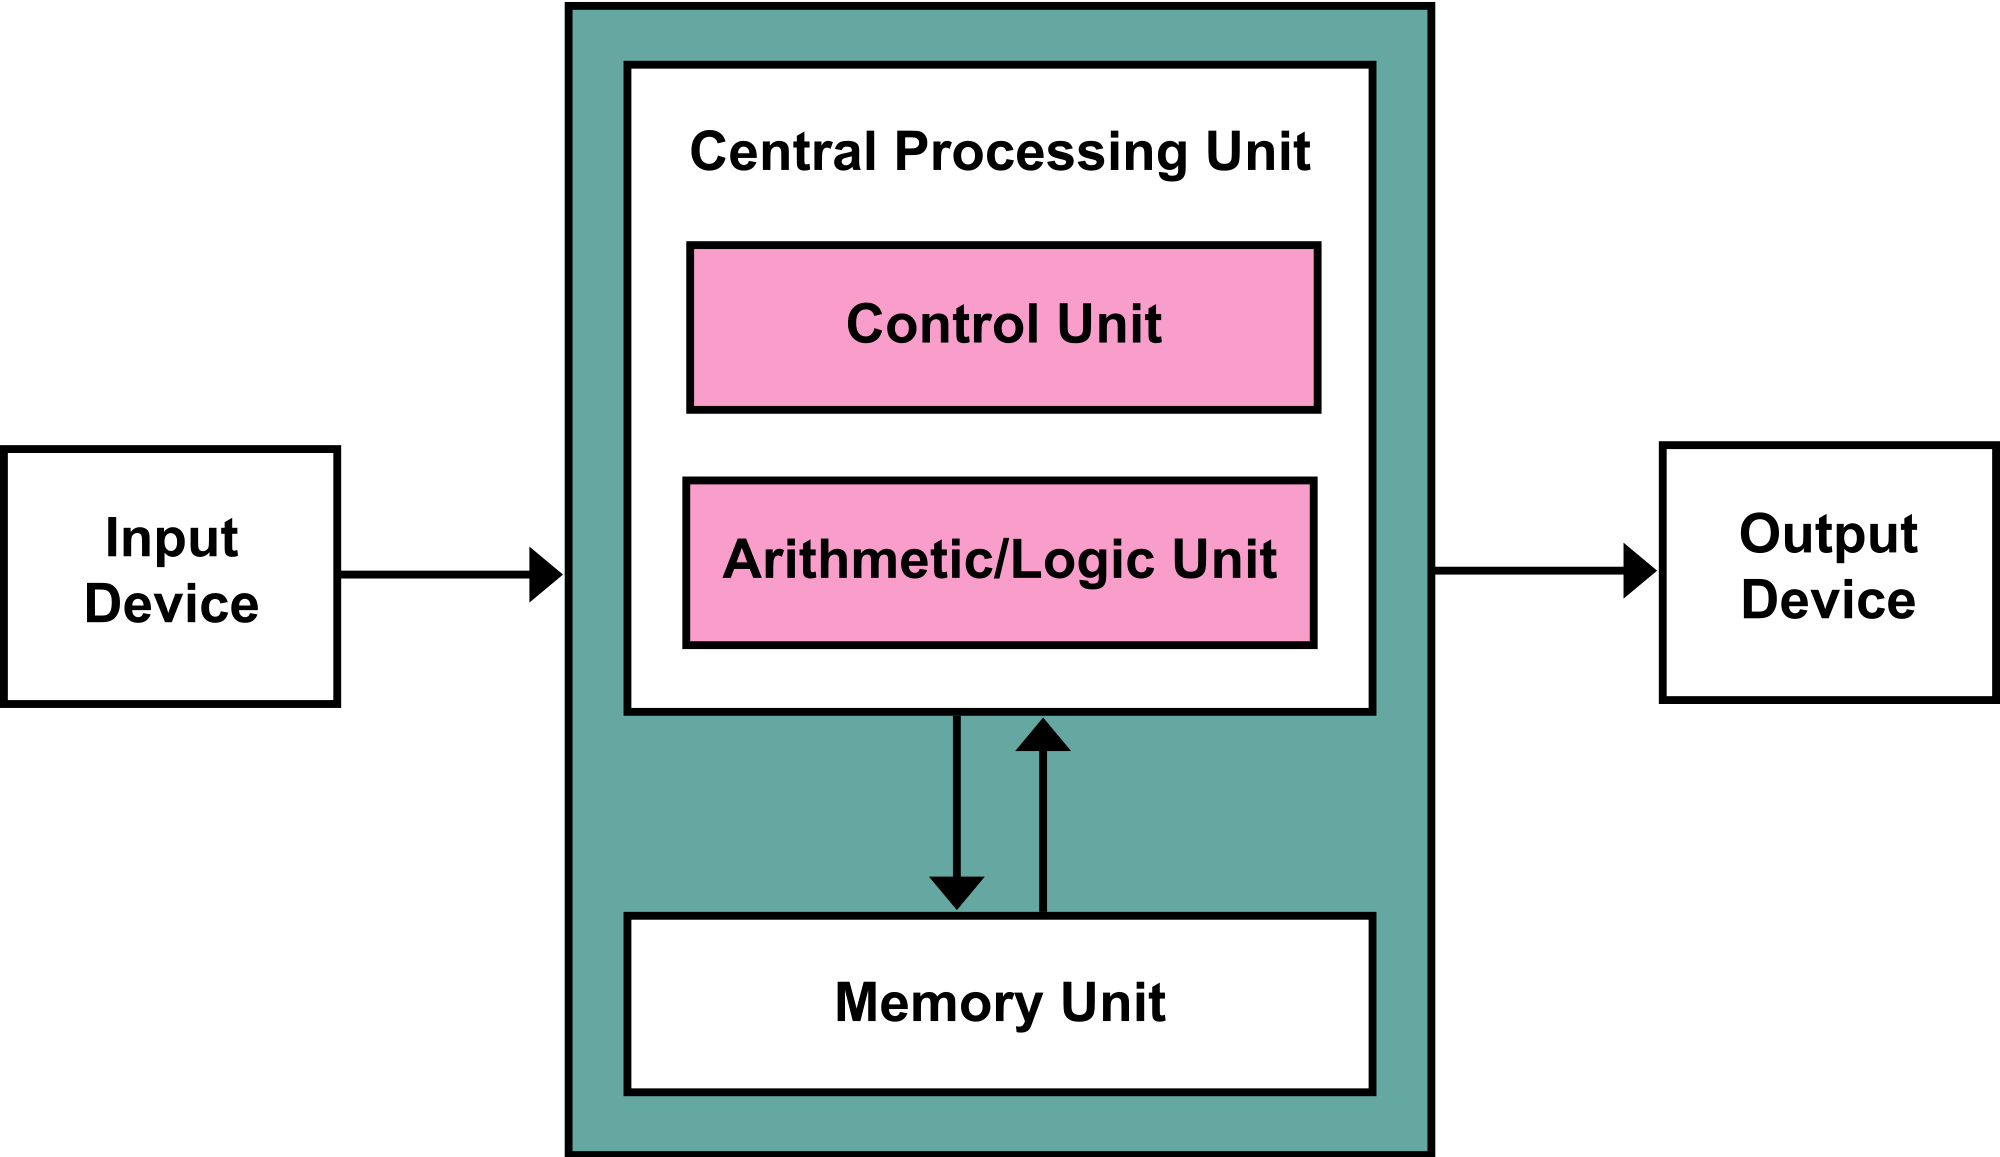
\includegraphics[width = 0.7\textwidth]{images/von_neumann.png}
    \label{fig:von_neumann}
    \caption{Von Neumann architecture scheme.}
\end{figure}

\begin{figure}
    \centering
    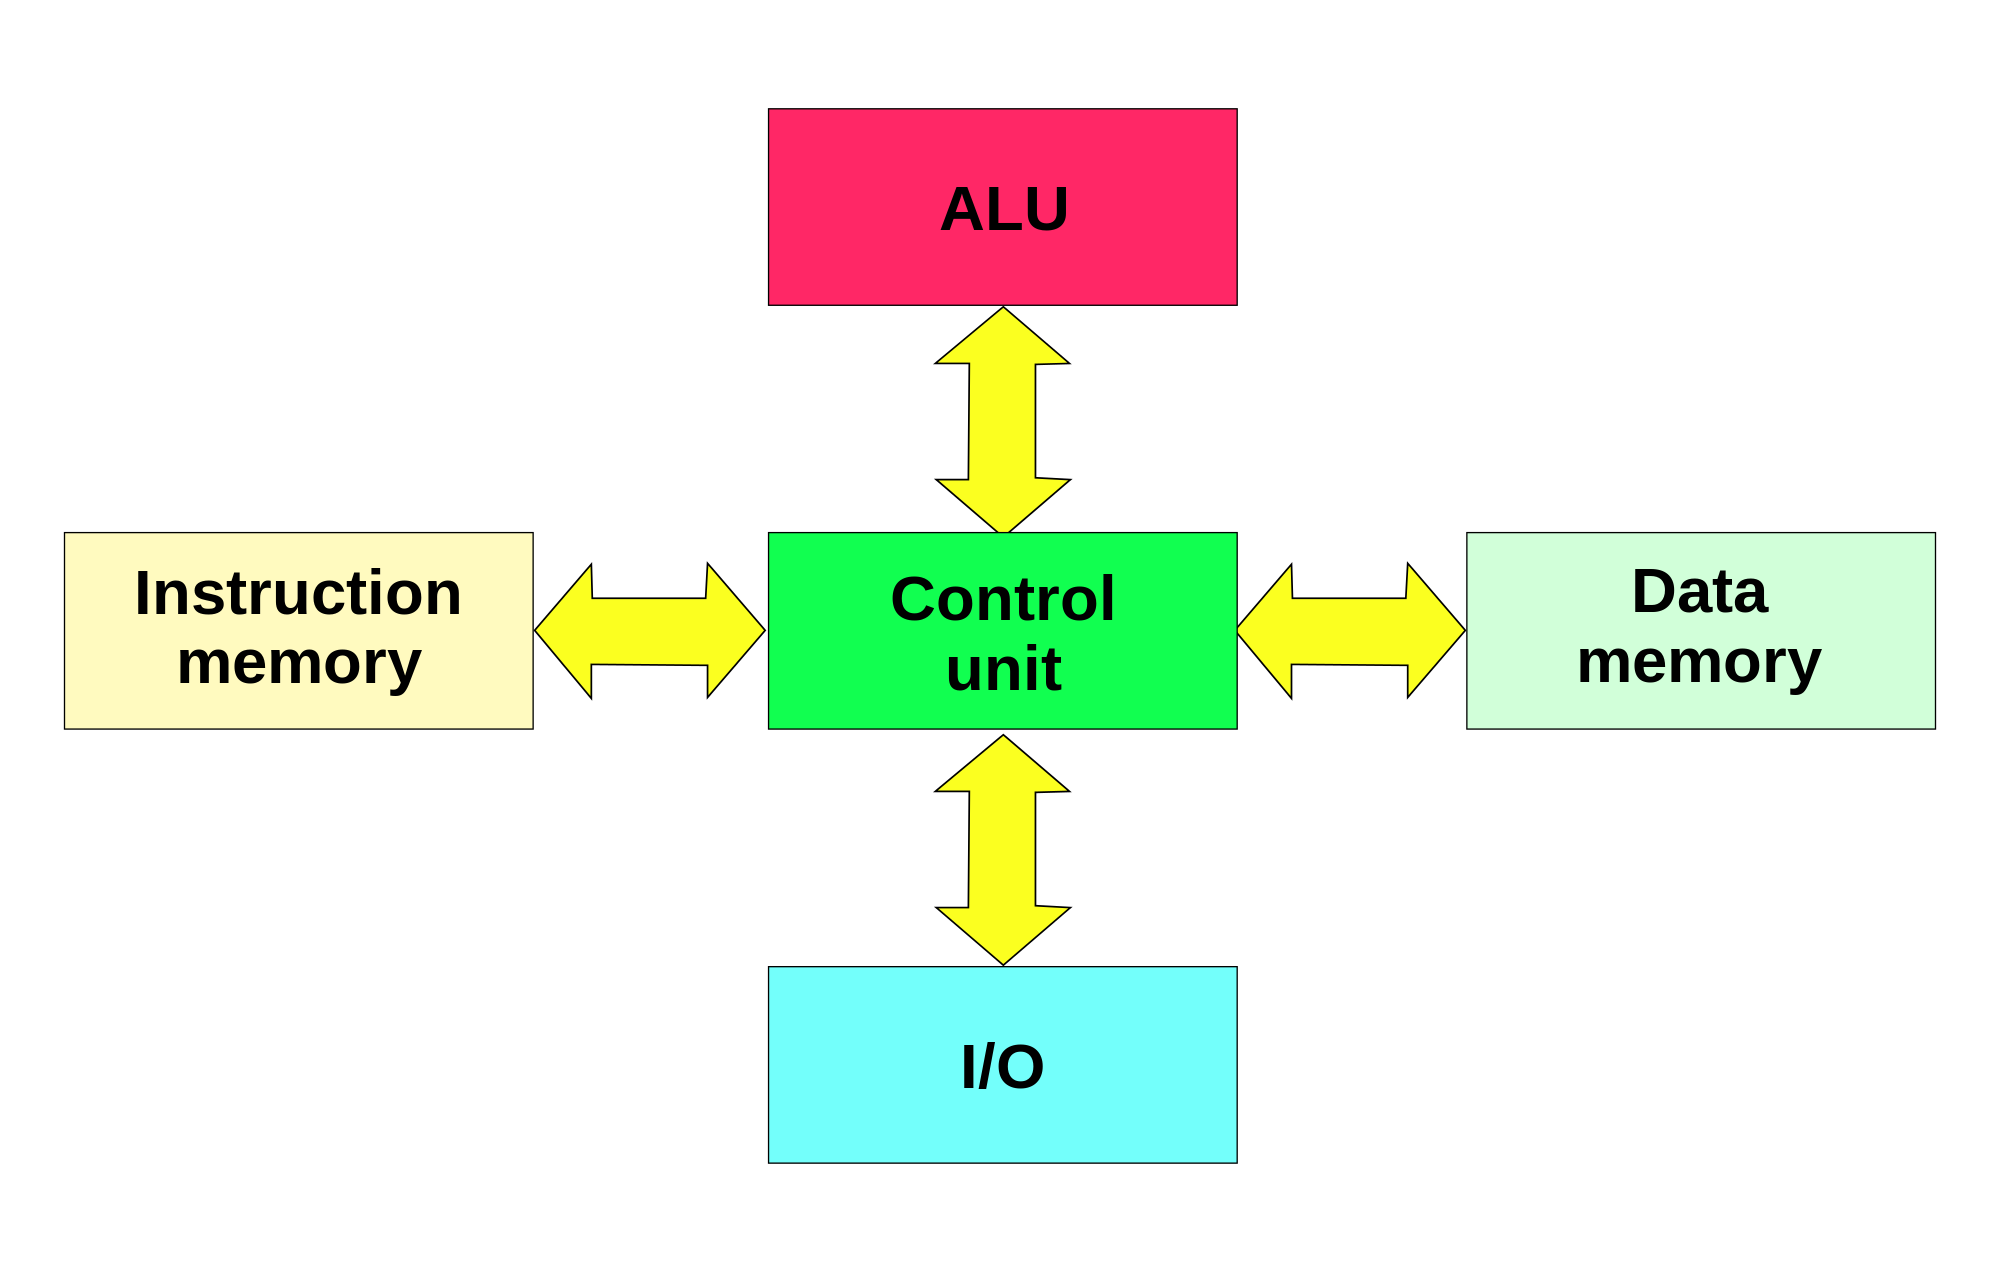
\includegraphics[width = 0.7\textwidth]{images/harvard.png}
    \label{fig:harvard}
    \caption{Harvard architecture scheme.}
\end{figure}

\begin{definition}[Von-Neumann architecture]
    \label{def:von_neumann}
    The \textbf{von Neumann architecture} is a fundamental computer architecture, the schema is shown in Figure \ref{fig:von_neumann}. It consists of
    \begin{enumerate}
        \item a processing unit that contains the datapath;
        \item a control unit;
        \item a memoroy unit that stores data and instructions;
        \item external mass storage; and
        \item input and output mechanisms. 
    \end{enumerate}
    There is a data bus and an instruction in between the memory unit and processing unit.
\end{definition}

A key aspect of von Neumann architecture is that the stored program (instructions) and data are both held in memory, this allows for self-modifying programs. However, what can arise from using this architecture is what we call the \textbf{von Neumann bottleneck}; that is, a limitation in the throughput between the central processing unit and the memory.

\begin{definition}[Harvard architecture]
    The \textbf{Harvard architecture} is another fundamental computer architecture, the schema is shown in Figure \ref{fig:harvard}. It consists of mainly the same components as the von Neumann architecture (Definition \ref{def:von_neumann}); however, the stored program and data and stored in separate arrays of memory. 
\end{definition}

The Harvard architecture allows us to fetch an instruction and fetch data simultaneously, which we could not do with von Neumann (without cache memory). This allows us to \textbf{pipeline}. This means that while we are fetching data for an instruction to execute, we can fetch the next instruction.

In practise, most computers use a \textbf{modified Harvard architecture} where, although data memory and instruction memory are separate, each with their own dedicated bus, the processor allows data to be treated as instructions and instructions to be treated as data; this allows for self-modifying or self-optimising code. In addition, there are separate CPU caches for instructions and data.

\begin{remark}
    The schema for von Neumann architecture and Harvard architecture (shown in Figure \ref{fig:von_neumann} and \ref{fig:harvard}) are simplified; in reality modern CPU architecture is considerably more complicated. These architectures just serve to describe some fundamental concepts.
\end{remark}

\begin{figure}
    \centering
    \makebox[\textwidth]{
        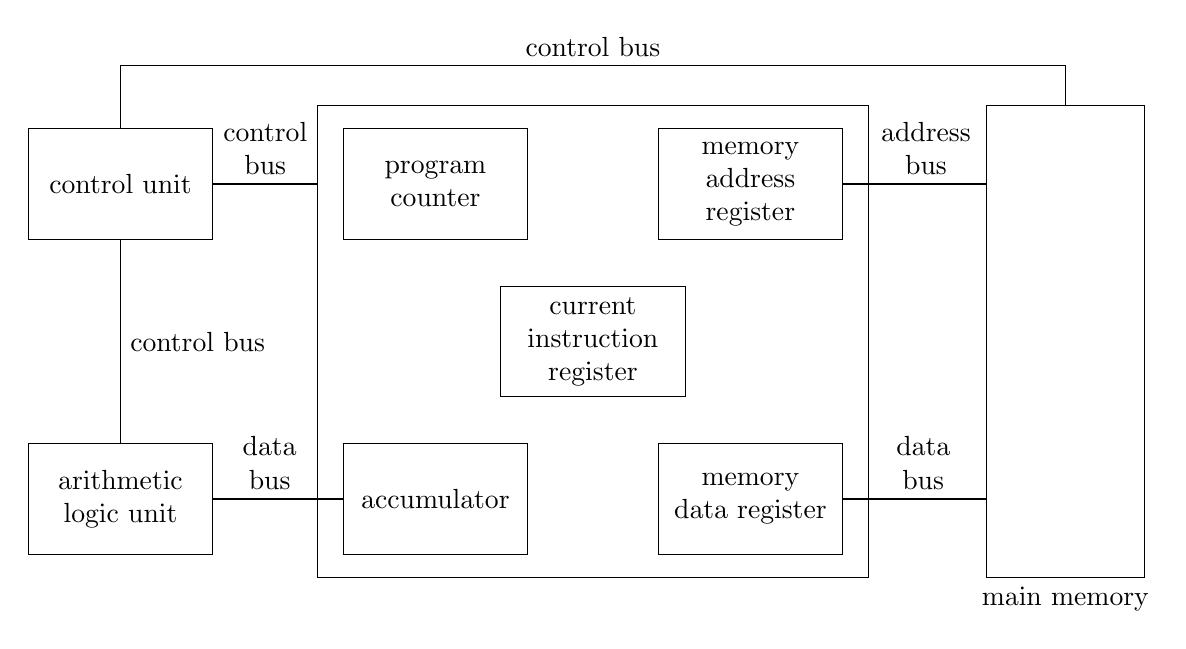
\begin{tikzpicture}
            \tikzstyle{box} = [rectangle, draw = black, text width = 6em, minimum width = 6em, minimum height = 4em, align = center]
            \node[box] at (0, 0) (alu) {arithmetic logic unit};
            \node[box] at (0, 4) (cu) {control unit};
            \node[box] at (4, 0) (acc) {accumulator};
            \node[box] at (4, 4) (pc) {program counter};
            \node[box] at (8, 0) (mdr) {memory data register};
            \node[box] at (8, 4) (mar) {memory address register};
            \node[box] at (6, 2) (cir) {current instruction register};
            \node[below] at (12, -1) {main memory};
            \draw (11, -1) rectangle (13, 5);
            \draw (2.5, -1) rectangle (9.5, 5);
            \draw (cu) -- (0, 5.5) -- node[above] {control bus} (12, 5.5) -- (12, 5);
            \draw (cu) -- node[right] {control bus} (alu);
            \draw (cu) -- node[above, align = center] {control \\ bus} (2.5, 4);
            \draw (alu) -- node[above, xshift = -3pt, align = center] {data \\ bus} (acc);
            \draw (mdr) -- node[above, xshift = 3pt, align = center] {data \\ bus} (11, 0);
            \draw (mar) -- node[above, xshift = 4pt, align = center] {address \\ bus} (11, 4);
        \end{tikzpicture}
    }
    \label{fig:basis_cpu}
    \caption{A basic processor architecture.}
\end{figure}

A basic processor architecture is shown in Figure \ref{fig:basis_cpu}. 

\begin{definition}[Fundamental components of a processor]
    The following are the fundamental components of a processor.
    \begin{enumerate}
        \item \textbf{Registers} are on-chip memory locations that are limited in number, according to the specification of the processor. This is the fastest way to access data.
        \item The \textbf{accumulator} is a special register which temporarily stores the results of arithmetic and logical operations.
        \item The \textbf{program counter} is a special register that holds the memory address where the next instruction can be found.
    \end{enumerate}
\end{definition}

\begin{definition}[Fetch-decode-fetch-execute cycle]
    Basic processor operations follows the \textbf{fetch-decode-fetch-execute} cycle as follows:
    \begin{enumerate}
        \item \textbf{instruction fetch}, the instruction address is supplied via the address bus and the data is returned via the data bus;
        \item \textbf{instruction decode}, the instruciton is interpreted;
        \item \textbf{operand fetch}, the address of any needed data is supplied via the address bus and then returned from memory via the data bus; and
        \item \textbf{execute instruction}, the instruction is performed, this step is typically followwed with a write-back where the output is written back to memory if needed.
    \end{enumerate}
\end{definition}

\begin{definition}[Instruction fetch]
    The CPU outputs the value of the program counter on the address bus, the memory reads the address bus and puts the content of the particular memory address onto the data bus. The instruction data is then stored in the current instruction register in the CPU.
\end{definition}

\begin{definition}[Instruction decode]
    The internally stored instruction data is decoded by the internal logic unit to provide the control signals to the ALU and other components of the CPU to execute the instruction. The program counter is then pushed onto the address bus and the ALU increments this value by the word-size and puts it back into the program counter. 
\end{definition}

\begin{definition}[Operand fetch]
    The instruction register proves the address of the data to be processed to the address bus. Memory supplies the operand data to the data bus, ready for processing by the ALU.
\end{definition}

\begin{definition}[Execute instruction]
    Processing is performed on the operand data in the ALU (or other processing unit) and the result (if any) is stored in the accumulator. The program counter here may be updated if there is a branch instruction or if the next instruction is in a different memory location than expected.
\end{definition}
